\clearpage


\chapter{Исследовательская часть}\label{ch:-}
В этом разделе приведен сравнительный анализ алгоритмов по количеству операций сравнения, необходимых для того, чтобы
найти искомый элемент в массиве.


\section{Технические характеристики ЭВМ}\label{sec:--2}
Все замеры проводились на ЭВМ, характеристики которой приведены ниже:
\begin{itemize}
    \item процессор: AMD Ryzen™ 7--5800H with Radeon™ Graphics × 16;
    \item ОС: 64-разрядная операционная система Ubuntu 24.04.1 LTS;
    \item оперативная память: 16,0 ГБ.
\end{itemize}


\section{Сравнение алгоритмов}
Размер массива, на котором проводилось исследование равен 1023, согласно варианту.
Предварительно массив был заполнен случайным образом с помощью модуля $random^{[2]}$.
Гистограммы построены с помощью библиотеки $matplotlib^{[3]}$.
Гистограммы \ref{grph:lsearch}--- \ref{grph:bsearch} показывают количество сравнений для каждого элемента словаря в линейном и бинарном поиске.
На рисунке \ref{grph:bsearch_sort} приведена отсортированная гистограмма из рисунка \ref{grph:bsearch}.

\begin{figure}
    \centering
    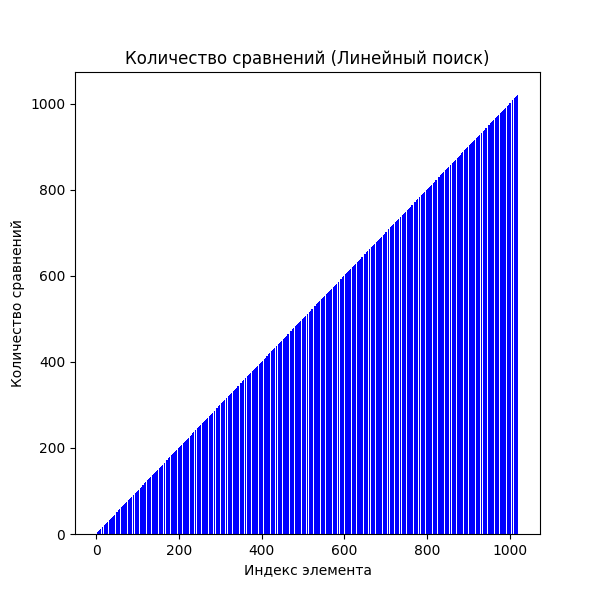
\includegraphics[width=1\linewidth]{images/ls}
    \caption{Сравнения для каждого элемента в алгоритме полного перебора}
    \label{grph:lsearch}
\end{figure}

\begin{figure}
    \centering
    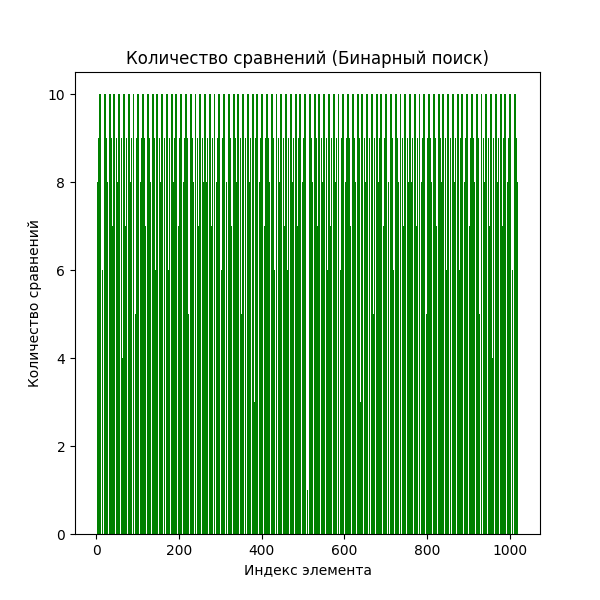
\includegraphics[width=1\linewidth]{images/bs}
    \caption{Сравнения для каждого элемента в алгоритме бинарного поиска}
    \label{grph:bsearch}
\end{figure}

\begin{figure}
    \centering
    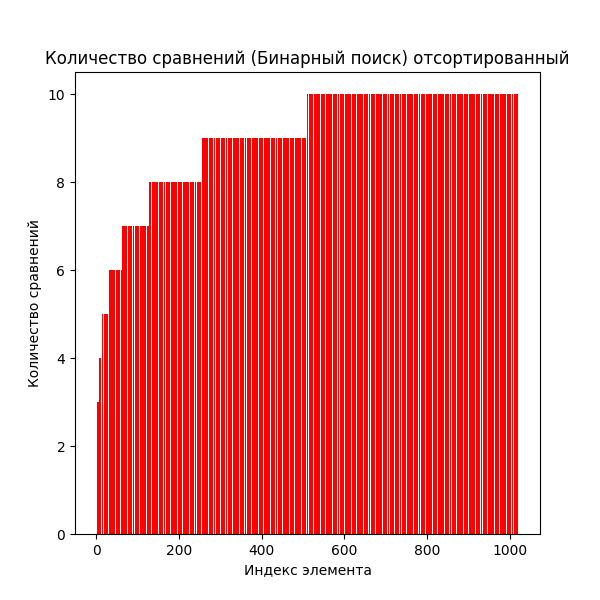
\includegraphics[width=1\linewidth]{images/bs_sort}
    \caption{Сравнения для каждого элемента в алгоритме бинарного поиска (отсортирован)}
    \label{grph:bsearch_sort}
\end{figure}

\clearpage
\section*{Вывод}

На основании анализа полученных гистограмм для двух алгоритмов поиска в массиве (линейного поиска и бинарного поиска) сделаны следующие выводы:

\textbf{Линейный поиск:}
В наилучшем случае, когда искомый элемент находится в начале массива, алгоритм выполняет минимальное количество операций, соответствующее трудоемкости $O(1)$. Как видно из гистограммы, количество операций увеличивается линейно с увеличением индекса элемента. Это полностью подтверждает теоретическую оценку трудоемкости алгоритма в худшем случае, равную $O(N)$, когда необходимо перебрать все элементы массива.

\textbf{Бинарный поиск:}
Для бинарного поиска в наилучшем случае (если элемент находится в середине массива) количество операций минимально и соответствует $O(1)$. Гистограмма демонстрирует, что количество сравнений меньше по сравнению с линейным поиском, особенно для элементов с высокими индексами. Трудоемкость алгоритма увеличивается логарифмически по мере увеличения индекса элемента, что подтверждает теоретическую оценку $O(\log N)$. В частности, при размере массива 1023 бинарный поиск завершает работу не более чем за 10 шагов, так как $2^{10} < 1023 < 2^{11}$. При этом, на малых индексах (до $7$) линейный поиск иногда оказывается эффективнее, так как для таких случаев требуется меньше операций, чем при первых шагах бинарного поиска.

\clearpage